\chapter{System Design}

\begin{figure}[!htbp]
	\centering
	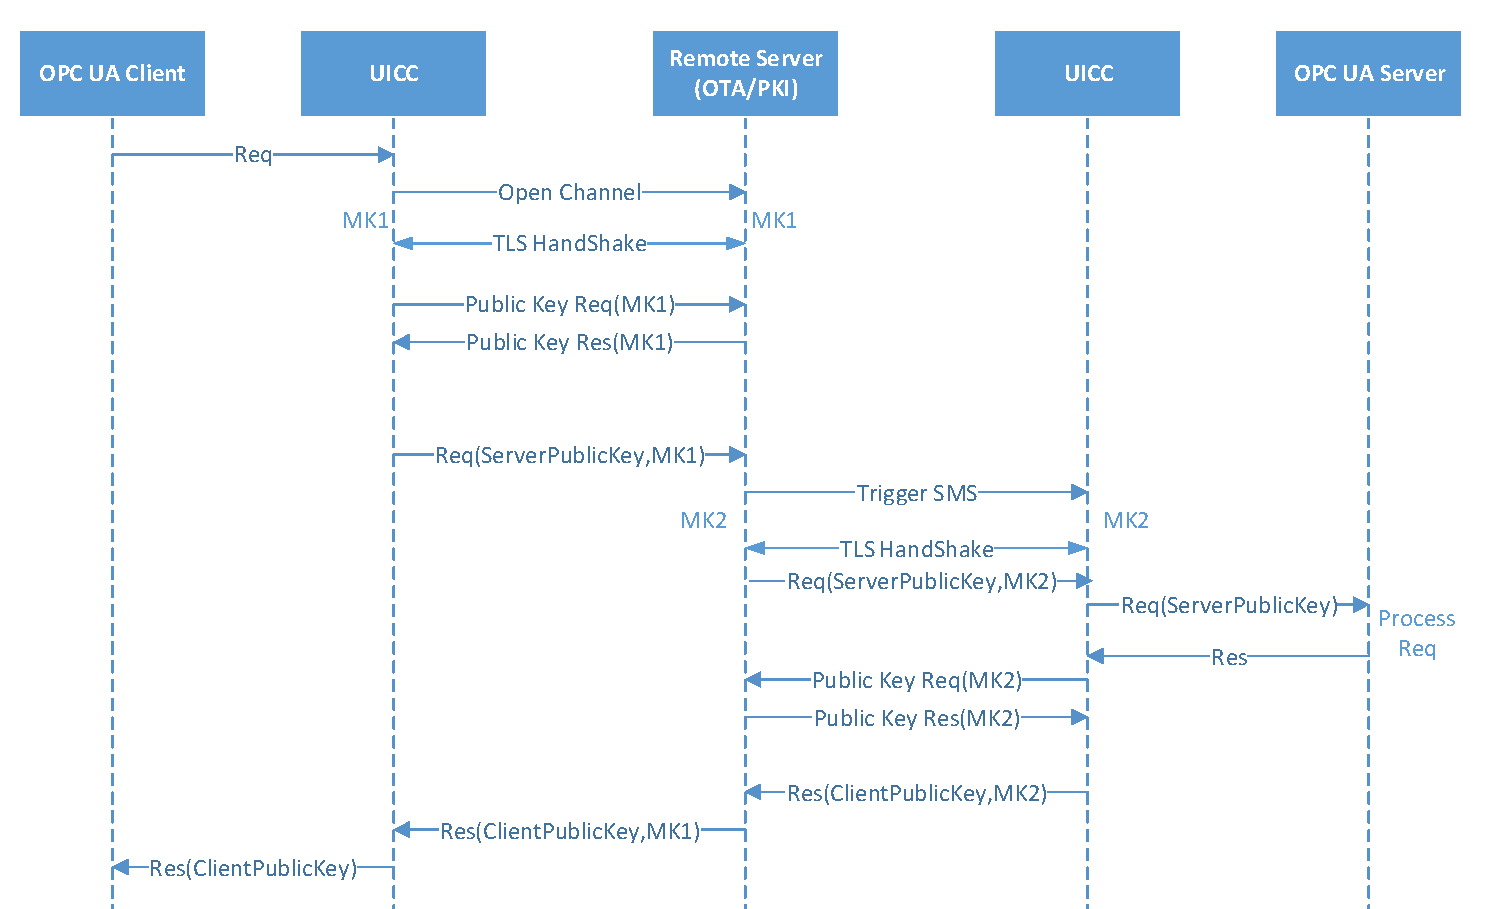
\includegraphics[width=1\textwidth]{whole-structure}
		\caption{Message Exchange}
	\label{fig:whole-structure}
\end{figure}

As described in previous sections, my demonstration system consists of three main parts, namely the on card integrated communication stack, Android application and Smart Home web service. Figure~\ref{fig:whole-structure} illustrates the request and corresponding response message exchange process that occurs in the demonstration system. In my case I integrate \emph{Public Key Infrastructure} with OTA server, in order to perform secure peer identification and messaging.


\section{UICC Applet}
\subsection{Overview}
The whole message exchange process consists of following phases:
\begin{itemize}
\item \emph{Open Channel Phase} Whenever a OPC UA client/server attempts to contact with other housing devices or Remote Server tries to communicate with a home device, a communication session between Remote Server and home device must be created.
\item \emph{TSL Handshake with Remote Server} After a successful creation of communication channel, a mutual peer identification through TLS handshake between Remote server and aforementioned client/server will be performed.
\item \emph{Require target's public key} When Remote Server identify the connected communication partner, it will grant client/server the expected target's public key. 
\item \emph{secure messaging} Message sender will in this phase encrypt message with target's public key and send this encrypted message through Remote Server to message receiver. 
\end{itemize}
\subsection {Work Flow}

The components involved in this scenario are:
 \begin{itemize}
  \item CommunicationStack applet and associated Security Domain from Globalplatform (APSD  for short)
  \item OTA server which is also known as Remote Administration Server (RAS for short)
\end{itemize}

The communication between CommunicationStack and Remote Administration Server involves following  steps:

 \begin{itemize}
  \item Open Communication Channel and Create Communication Session
  \item Secure Message Exchange
  \item Close Communication Session
\end{itemize}
\subsubsection{Communication Session Creation and Message Exchange}
This process could be either initiated by Remote Administration Server by sending target applet a trigger SMS or be sponsored by applet itself. In both cases, applet sends the first \emph{OpenChannel Request} message. During the PSK TLS Handshake phase, APSD and remote server will agree on to be used cipher suit and authenticate each other. After a successful PSK TLS Handshake, CommunicationStack and remote OTA server will be able to exchange HTTP message, which encapsulates APDU strings as body. And HTTP header is in compliance with GlobalPlatform standards.


\begin{figure}[!htbp]

	\centering
	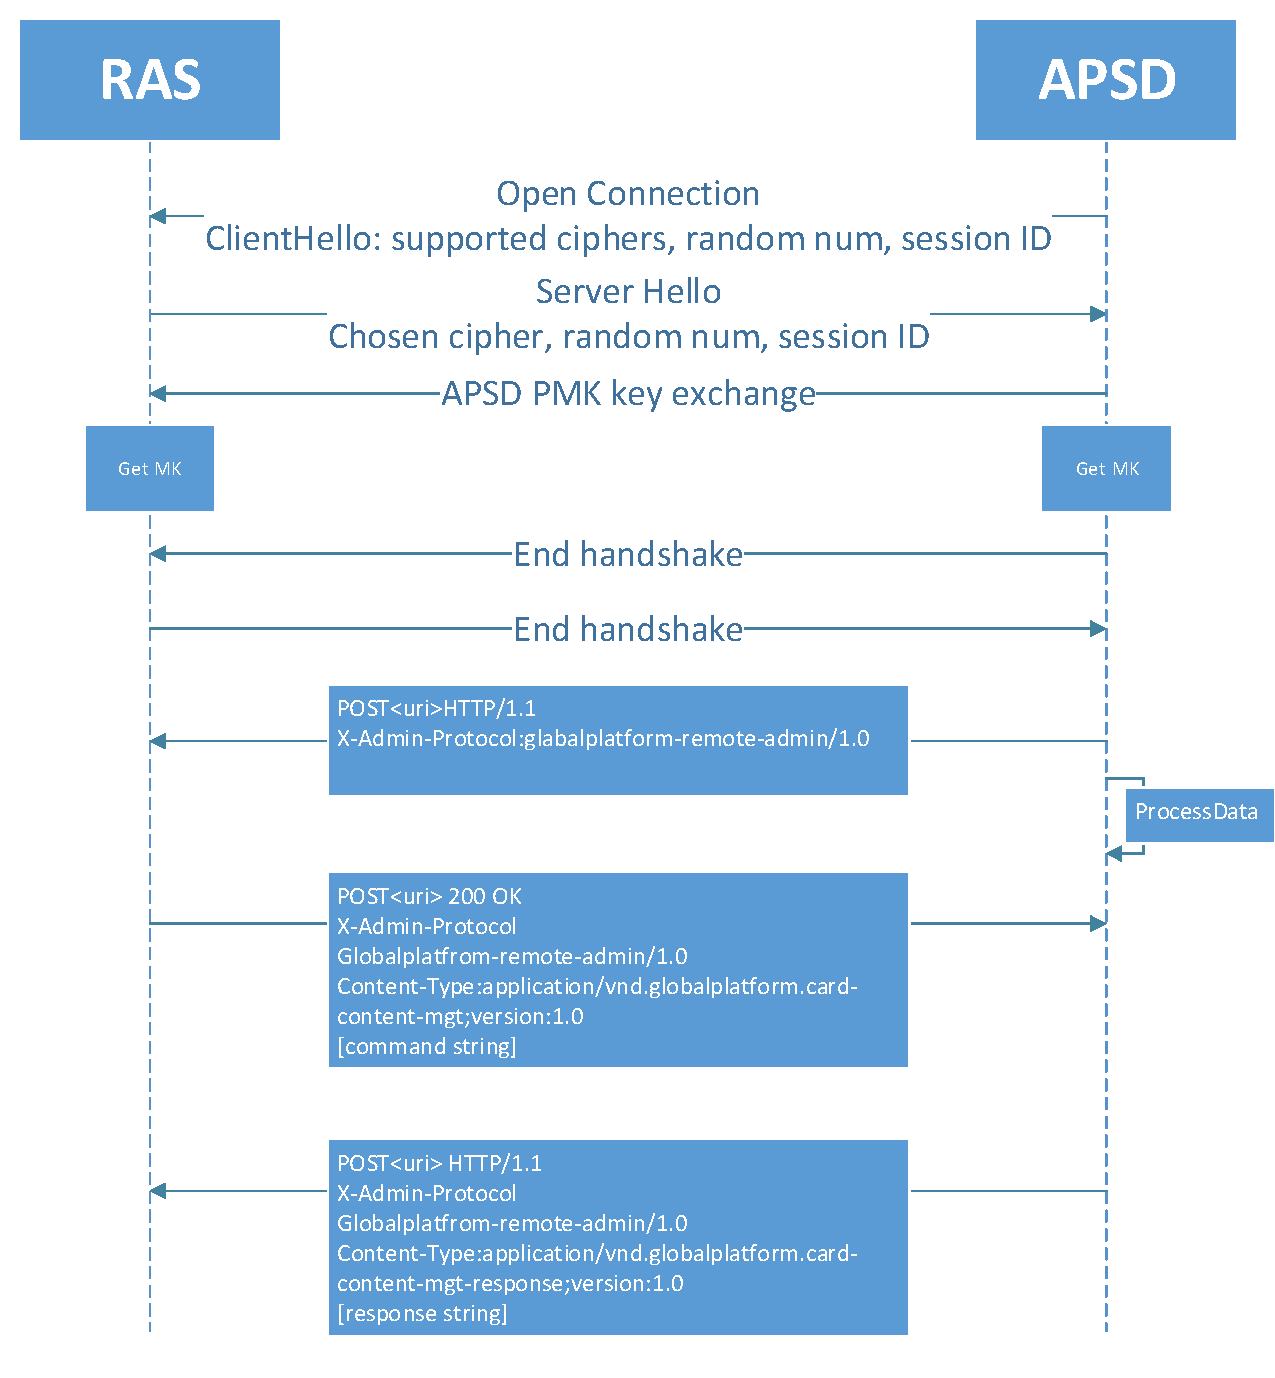
\includegraphics[width=1\textwidth]{communication-flow}
		\caption{Handshake and message exchange between SD and Remote Server}
	\label{fig:communication-flow}
\end{figure}

\subsubsection{HTTP Header Format}
The HTTP message sent from remote sever to targeted applet uses following schema\cite{gp}:
\begin{Verbatim}[fontsize=\relsize{-1}, frame=lines,framesep=4mm, label=\fbox{\small\emph{Http Request Schema}}]
HTTP/1.1 200 OK [or HTTP/1.1 204 No Content CRLF]
X-Admin-Protocol: globalplatform-remote-admin/1.0 CRLF
[X-Admin-Next-URI:  <next-URI> CRLF]
[Content-Type: application/vnd.globalplatform.card-content-mgt
-response;version=1.0 CRLF]
[X-Admin-Targeted-Application: <security-domain-AID> CRLF]
[Content-Length: xxxx CRLF] or [Transfer-Encoding: chunked CRLF]
CRLF
[body]
\end{Verbatim}
The field \emph{security-domain-AID} will be filled with the AID of targeted applet.


The HTTP response message sent from applet to remote server uses following schema\cite{gp}:
\begin{Verbatim}[fontsize=\relsize{-1}, frame=lines,framesep=4mm, label=\fbox{\small\emph{Http Response Schema}}]
POST<URI>HTTP/1.1 CRLF
Host: <Administration Host> CRLF
X-Admin-Protocol: globalplatform-remote-admin/1.0 CRLF
X-Admin-From: <Agent ID> CRLF
[Content-Type: application/vnd.globalplatform.card-content-mgt
-response;version=1.0 CRLF]
[Content-Length: xxxx CRLF] or [Transfer-Encoding: chunked CRLF]
[X-Admin-Script-Status: <script-status> CRLF]
[X-Admin-Resume: true]
CRLF
[body]
\end{Verbatim}

The filed \emph{X-Admin-Script-Status} could contain following values:
 \begin{itemize}
  \item \emph{ok}, which means that the previous message is successfully received by applet.
  \item \emph{unknown-application}, which stands for the error, that the targeted applet for previous message can not be found.
\item \emph{not-a-security-domain}, this errors occurs when targeted applet is not a Security Domain.
\item \emph{security-error}, as its name indicates, this values is returned if the security of previous message  can not be checked.
\end{itemize}

\subsubsection{Close Communication Session}
Whenever the communication channel is about to be closed, either because of session security issue, or due to successful finish of communication, remote server will send target applet HTTP message using following parameters:
 \begin{itemize}
  \item No \emph{X-Admin-Next-URI} field is present in this HTTP message and message body is empty, which will be recognized as final message from remote server and then the session will be closed.
  \item No \emph{X-Admin-Next-URI} filed is present but in this HTTP message body is not empty. The receiver will process the data in body and close the communication session appropriately. But no response message will be generated.
\end{itemize}

\subsection {Commands: Interface between Applet and CAD} \label{secAPDU}
Before concrete implementation of Javacard applet code, the interface, which in essence is a set of commond APDUs and corresponding response APDUs, between applet and CAD must be well defined.  The CommunicationStack support two categories commond APDU:
 \begin{itemize}
  \item The \emph{SELECT} Command APDU, which is used by JCRE to select CommunicationStack applet.
  \item Other command APDUs, which are introduced in order to provide functionalists such as: trigger communication session, process input APDU and etc. To be more specifically:
\begin{itemize}
  \item PIN operation related APDU set
  \item Communication session management APDU set
  \item Data process APDU set
\end{itemize}
\end{itemize}

\subsubsection{SELECT APDU}
The header of this command APDU is fixed and \emph{Lc} indicates the length of CommunicationStack AID. In \emph{Data filed} real AID is saved.
\begin{table}[!htbp]
\caption{SELECT command APDU}
\scalebox{0.8}{%
\begin{tabular}{|l|l|l|l|l|l|l|}
\hline
CLA  & INS  & P1   & P2   & Lc   & Data field                                                                                          & Le  \\ \hline
0x00 & 0xA4 & 0x04 & 0x00 & Length of AID& AID & N/A \\ \hline
\end{tabular}
}
\label{select-apdu}
\end{table}
Two categories of response APDUs are expected, one represents successful processing of \emph{SELECT} command APDU and the other stands for failure.
\begin{table}[!htbp]
\caption{SELECT response APDU}
\label{select-response-apdu}
\scalebox{0.8}{%
\begin{tabular}{|l|l|l|}
\hline
Optional data & Status word & Description                                \\ \hline
No data       & 0x9000      & Successful processing                      \\ \hline
              & 0x6999      & Failed to select CommunicationStack applet \\ \hline               
\end{tabular}
}
\end{table}

\subsubsection{Verify PIN operation}
This APDU command and response set is used to let CommunicationStack applet verify identity of terminal user. Moreover the PIN size is set from four to eight and the verify PIN operation only allows three times wrong PIN input before a successful identification.

\begin{table}[!htbp]
\caption{Verify PIN command }
\scalebox{0.8}{%
\begin{tabular}{|l|l|l|l|l|l|l|}
\hline
CLA  & INS  & P1   & P2   & Lc   & Data field    & Le  \\ \hline
0xA0 & 0x11 & 0x00 & 0x00 & length of Data field & PIN & N/A \\ \hline
\end{tabular}
}
\label{verify-command-apdu}
\end{table}

As described in tabl~\ref{verify-response-apdu}, three categories of response APDUs are expected.

\begin{table}[!htbp]
\caption{Verify PIN response APDU}
\label{verify-response-apdu}
\scalebox{0.8}{%
\begin{tabular}{|l|l|l|}
\hline
Optional data & Status word & Description                                \\ \hline
No data       & 0x9000      & Successful processing                      \\ \hline
              & 0x63C0      & Verification failed \\ \hline      
              & 0x6983      & After 3 times wrong input, PIN is block \\ \hline              
\end{tabular}
}
\end{table}

\subsubsection{Reset PIN operation}
This APDU command and response set is introduced to offer end user change PIN service.

\begin{table}[!htbp]
\caption{Reset PIN command }
\scalebox{0.8}{%
\begin{tabular}{|l|l|l|l|l|l|l|}
\hline
CLA  & INS  & P1   & P2   & Lc   & Data field    & Le  \\ \hline
0xA0 & 0x12 & 0x00 & 0x00 & length of Data field &New PIN & N/A \\ \hline
\end{tabular}
}
\label{reset-pin-command-apdu}
\end{table}

Three categories of response APDUs are expected.
\begin{table}[!htbp]
\caption{Reset PIN response APDU}
\label{reset-pin-response-apdu}
\scalebox{0.8}{%
\begin{tabular}{|l|l|l|}
\hline
Optional data & Status word & Description                                \\ \hline
No data       & 0x9000      & Successful processing                      \\ \hline
              & 0x6301      & Verification is required first\\ \hline      
              & 0x6984      & Length of input PIN is wrong \\ \hline              
\end{tabular}
}
\end{table}


\subsubsection{Communication Session Creation}\label{secSessionOpen}
\begin{table}[!htbp]
\caption{Communication session creation command APDUs}
\scalebox{0.75}{%
\begin{tabular}{|l|l|l|l|l|l|l|l|}
\hline
CLA  & INS  & P1   & P2   & Lc   & Data field  & Le  & Description \\ \hline
0xA0 & 0x01 & 0x00 & 0x00 & data filed length & Session parameter& N/A  & create session parameters\\ \hline
0xA0 & 0x02 & 0x00 & 0x00 & data filed length & Session parameter& N/A  & set session parameters\\ \hline
0xA0 & 0x03 & 0x00 & 0x00 &  N/A & N/A& N/A  & create communication session\\ \hline
0xA0 & 0x04 & 0x00 & 0x00 &  N/A & N/A& length of session state & get session state\\ \hline
\end{tabular}
}
\label{trigger-session-apdu}
\end{table}
This APDU command and response set is used to let  CommunicationStack applet initiate the request to establish communication channel and create communication  session above  it. Following commands are supported.



Following return codes are expected in response APDU:

.\begin{table}[!htbp]
\caption{Trigger Session Return Code}
\label{trigger-session-response-apdu}
\scalebox{0.8}{%
\begin{tabular}{|l|l|l|}
\hline
 Status word & Description                                \\ \hline
 0x9000      & Successful processing                      \\ \hline
 0x66AB      & Array Index out of bounds exception \\ \hline           
 0x665E      & Security exception \\ \hline 
 0x6600      & Nullpointer  exception \\ \hline  
 0x6C00      & UnKnown  exception \\ \hline      
\end{tabular}
}
\end{table}


\subsubsection{Close Communication Session}\label{secSessionClose}
This APDU command and response set is used to correctly close  communication channel.


\begin{table}[!htbp]
\caption{Close Session command APDU}
\scalebox{0.8}{%
\begin{tabular}{|l|l|l|l|l|l|l|}
\hline
CLA  & INS  & P1   & P2   & Lc   & Data field                                                                                          & Le  \\ \hline
0xA0 & 0x50 & 0x00 & 0x00 & 0x00 & N/A& N/A \\ \hline
\end{tabular}
}
\label{close-session-apdu}
\end{table}

Following return codes are expected in response APDU:

.\begin{table}[!htbp]
\caption{Close Session Return Code}
\label{close-session-response-apdu}
\scalebox{0.8}{%
\begin{tabular}{|l|l|l|}
\hline
 Status word & Description                                \\ \hline
 0x9000      & Successful processing                      \\ \hline
 0x6032      & Failed to close session \\ \hline             
\end{tabular}
}
\end{table}

\subsubsection{Process Communication Data }\sloppy
\begin{table}[!htbp]
\caption{Process data command APDUs}
\scalebox{0.8}{%
\begin{tabular}{|l|l|l|l|l|l|l|l|}
\hline
CLA  & INS  & P1   & P2   & Lc   & Data field  & Le \\ \hline
0xA0 & 0x20 & 0x00 & 0x00 & data filed length & desired target's public key & PK length \\ \hline
0xA0 & 0x21 & 0x00 & 0x00 & data filed length & command data & response length \\ \hline
\end{tabular}
}
\label{process-data-cmd-apdu}
\end{table}
This APDU command and response set is used to provide functionalities to perform command processing between cellphone and  other smart home device. 

\begin{table}[!htbp]
\caption{Process data Return Code}
\label{process-data-res-apdu}
\scalebox{0.8}{%
\begin{tabular}{|l|l|l|}
\hline
 Status word & Description                                \\ \hline
 0x9000      & Successful processing                      \\ \hline
 0x6A80      & error in data filed \\ \hline        
 0x6A81      & required device not found \\ \hline        
 0x6A82      & required service not found \\ \hline   
 0x6A83      & required record not found \\ \hline                
\end{tabular}
}
\end{table}
Following return codes as shown in table~\ref{process-data-res-apdu} are expected in response APDU.

Moreover \emph{command data} in data filed of command APDU adopts following TLV format as shown in table~\ref{tlv}. 
% Please add the following required packages to your document preamble:
% \usepackage{multirow}
% \usepackage{graphicx}
\begin{table}[!htbp]
\resizebox{\textwidth}{!}{%
\begin{tabular}{|l|l|l|l|l|l|l|l|l|l|}
\hline
Tag & Length & \multicolumn{7}{l|}{Name} & Presence \\ \hline
'90' & 0-n & \multicolumn{7}{l|}{command parameters} & \multirow{2}{*}{optional} \\ \cline{1-9}
\multicolumn{2}{|l|}{\multirow{30}{*}{}} & Tag & Length & \multicolumn{5}{l|}{Name} &  \\ \cline{3-10} 
\multicolumn{2}{|l|}{} & '91' & 0-n & \multicolumn{5}{l|}{command from cell phone to home device} & \multirow{2}{*}{optional} \\ \cline{3-9}
\multicolumn{2}{|l|}{} & \multicolumn{2}{l|}{\multirow{18}{*}{}} & Tag & Length & \multicolumn{3}{l|}{Name} &  \\ \cline{5-10} 
\multicolumn{2}{|l|}{} & \multicolumn{2}{l|}{} & '92' & 1-n & \multicolumn{3}{l|}{Read sensor value} & optional \\ \cline{5-10} 
\multicolumn{2}{|l|}{} & \multicolumn{2}{l|}{} & \multicolumn{2}{l|}{\multirow{2}{*}{}} & Tag & Length & Name & \multirow{2}{*}{} \\ \cline{7-9}
\multicolumn{2}{|l|}{} & \multicolumn{2}{l|}{} & \multicolumn{2}{l|}{} & '9C' & 1-n & device uid &  \\ \cline{5-10} 
\multicolumn{2}{|l|}{} & \multicolumn{2}{l|}{} & '93' & 1-n & \multicolumn{3}{l|}{Set subscription} & optional \\ \cline{5-10} 
\multicolumn{2}{|l|}{} & \multicolumn{2}{l|}{} & \multicolumn{2}{l|}{\multirow{2}{*}{}} & Tag & Length & Name & \multirow{3}{*}{} \\ \cline{7-9}
\multicolumn{2}{|l|}{} & \multicolumn{2}{l|}{} & \multicolumn{2}{l|}{} & '9C' & 1-n & sensor uid &  \\ \cline{5-9}
\multicolumn{2}{|l|}{} & \multicolumn{2}{l|}{} &  &  & '9A' & 1-256 & subscription value &  \\ \cline{5-10} 
\multicolumn{2}{|l|}{} & \multicolumn{2}{l|}{} & '94' & 1-n & \multicolumn{3}{l|}{Get historical record} & optional \\ \cline{5-10} 
\multicolumn{2}{|l|}{} & \multicolumn{2}{l|}{} & \multicolumn{2}{l|}{\multirow{2}{*}{}} & Tag & Length & Name & \multirow{2}{*}{} \\ \cline{7-9}
\multicolumn{2}{|l|}{} & \multicolumn{2}{l|}{} & \multicolumn{2}{l|}{} & '9C' & 1-n & device uid &  \\ \cline{5-10} 
\multicolumn{2}{|l|}{} & \multicolumn{2}{l|}{} & '95' & 1 & \multicolumn{3}{l|}{Open main door} & optional \\ \cline{5-10} 
\multicolumn{2}{|l|}{} & \multicolumn{2}{l|}{} & '96' & 1 & \multicolumn{3}{l|}{Coffee Maker add water} & optional \\ \cline{5-10} 
\multicolumn{2}{|l|}{} & \multicolumn{2}{l|}{} & '97' & 1 & \multicolumn{3}{l|}{Coffee Maker add coffee} & optional \\ \cline{5-10} 
\multicolumn{2}{|l|}{} & \multicolumn{2}{l|}{} & '98' & 1 & \multicolumn{3}{l|}{Coffee Maker make coffee} & optional \\ \cline{5-10} 
\multicolumn{2}{|l|}{} & \multicolumn{2}{l|}{} & '99' & 1-n & \multicolumn{3}{l|}{Grant main door access to} & optional \\ \cline{5-10} 
\multicolumn{2}{|l|}{} & \multicolumn{2}{l|}{} & \multicolumn{2}{l|}{\multirow{2}{*}{}} & Tag & Length & Name & \multirow{2}{*}{} \\ \cline{7-9}
\multicolumn{2}{|l|}{} & \multicolumn{2}{l|}{} & \multicolumn{2}{l|}{} & '9B' & 1-n & user uid &  \\ \cline{3-10} 
\multicolumn{2}{|l|}{} & '9D' & 0-n & \multicolumn{5}{l|}{Command from home device to cell phone} & \multirow{2}{*}{optional} \\ \cline{3-9}
\multicolumn{2}{|l|}{} & \multicolumn{2}{l|}{\multirow{9}{*}{}} & Tag & Length & \multicolumn{3}{l|}{Name} &  \\ \cline{5-10} 
\multicolumn{2}{|l|}{} & \multicolumn{2}{l|}{} & '9E' & 0-n & \multicolumn{3}{l|}{Notification sent by home device} & optional \\ \cline{5-10} 
\multicolumn{2}{|l|}{} & \multicolumn{2}{l|}{} & \multicolumn{2}{l|}{\multirow{3}{*}{}} & Tag & Length & Name & \multirow{3}{*}{} \\ \cline{7-9}
\multicolumn{2}{|l|}{} & \multicolumn{2}{l|}{} & \multicolumn{2}{l|}{} & '9C' & 1-n & device uid &  \\ \cline{7-9}
\multicolumn{2}{|l|}{} & \multicolumn{2}{l|}{} & \multicolumn{2}{l|}{} & '9A' & 1-256 & value &  \\ \cline{5-10} 
\multicolumn{2}{|l|}{} & \multicolumn{2}{l|}{} & '9F' & 0-n & \multicolumn{3}{l|}{Historical data} & optional \\ \cline{5-10} 
\multicolumn{2}{|l|}{} & \multicolumn{2}{l|}{} & \multicolumn{2}{l|}{\multirow{3}{*}{}} & Tag & Length & Name & \multirow{3}{*}{} \\ \cline{7-9}
\multicolumn{2}{|l|}{} & \multicolumn{2}{l|}{} & \multicolumn{2}{l|}{} & '9C' & 1-n & device uid &  \\ \cline{7-9}
\multicolumn{2}{|l|}{} & \multicolumn{2}{l|}{} & \multicolumn{2}{l|}{} & ''A0' & 1-256 & historical data &  \\ \hline
\end{tabular}
}
\caption{Command data Type-Length-Value structure}
\label{tlv}
\end{table}
Based on above described TLV structure, following APDU \emph{A0210000129010910892069C040102030402}\label{remote-apdu-example} can be translated as command sent by smart phone to sensor with \emph{uid 01020304} for the purpose of querying current sensor value. And the expected response data length is set as two bits. Any ill-formed command data will be ignored.

\subsection{Classes}\sloppy
My UICC applet is integrated in Morpho \emph{SC5-01OS07} LTE SAT product and contains following classes:
 \begin{itemize}
  \item  \emph{CommunicationStack}, which is the main class of my applet, that implements \emph{install}, \emph{select}, \emph{deselect} as well as \emph{process} methods provided by \emph{javacard.framework.Applet}. In order to process remote APDU, this applet is also designed as UICC system applet, that extends interface \emph{com.orga.javacard.componentinterfaces.JCISIMApplication}
  \item  \emph{sessionTrigger}, which implements Globalplatform  and toolkitframework interfaces and offers functions for proactive and passive communication session creation with OTA server, cipher suit negotiation and mutual authentication. \emph{sessionTrigger} is developed based on \emph{adminTrigger} class provided by Morpho.
\end{itemize}

\begin{figure}[!htbp]
	\centering
	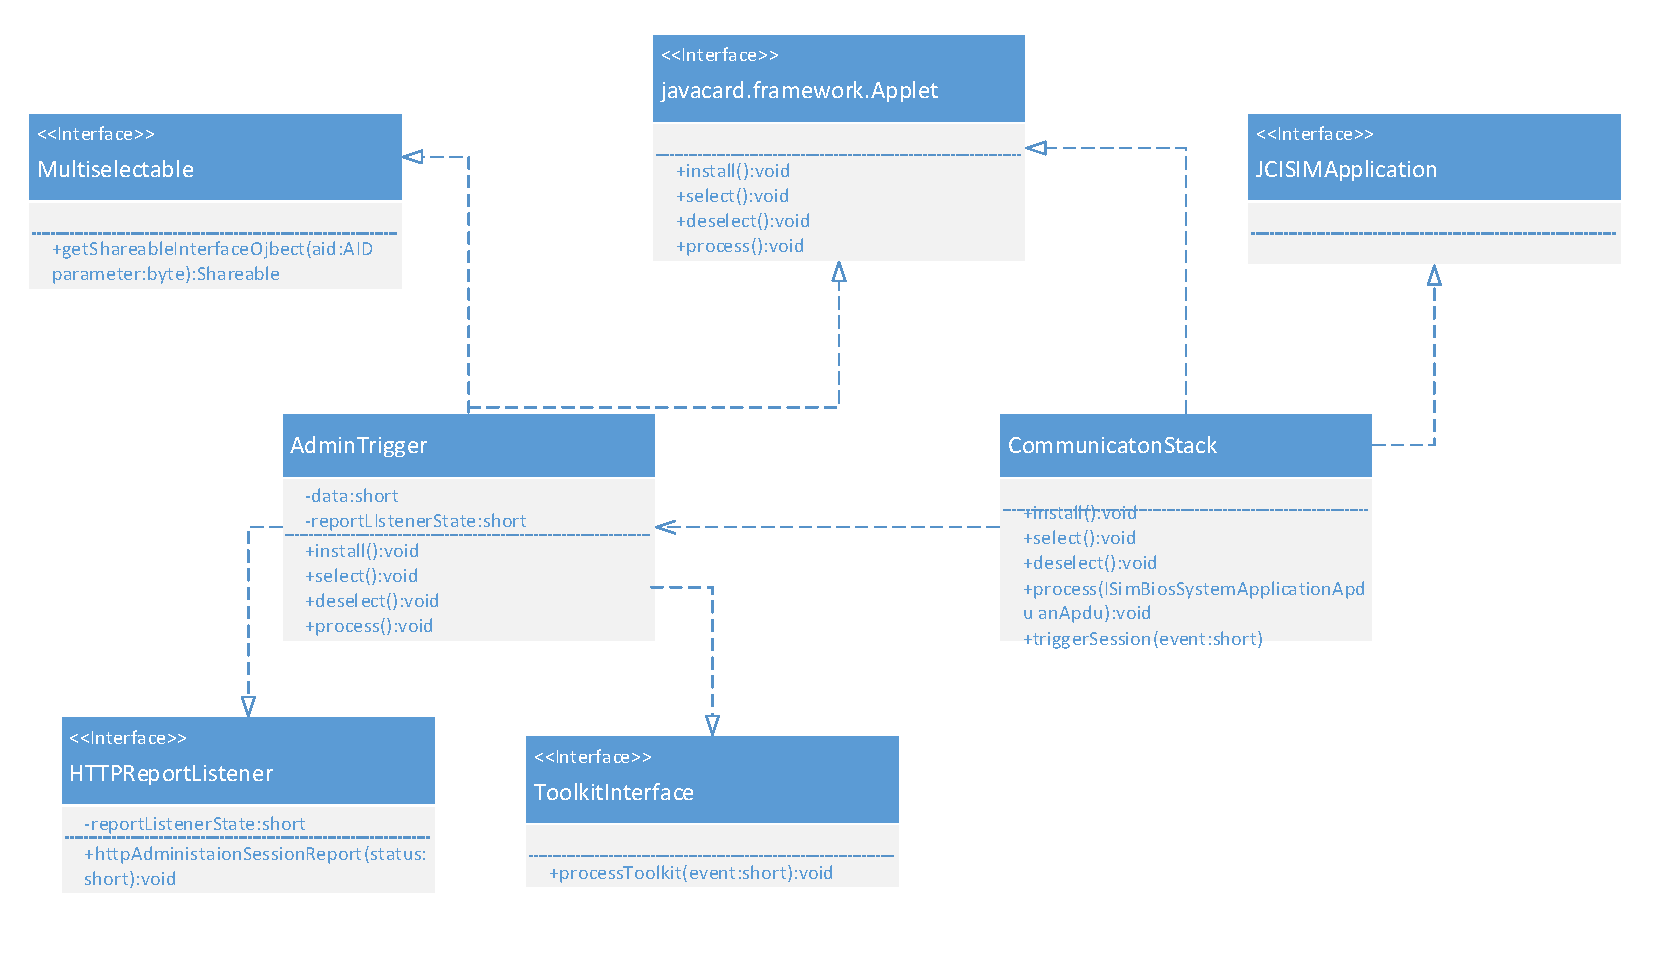
\includegraphics[width=1.0\textwidth]{class}
		\caption{Class Diagram}
	\label{fig:class}
\end{figure}

\subsubsection{Class CommunicationStack} \sloppy
As the main class of my Applet, \emph{communicationStack} extends \emph{UsimRemoteService} class provided by Morpho in order to be recognized as a system Applet, which is capable of performing remote file management behavior. Moreover this main class has implemented interface \emph{JCISIMApplication}, which defines how to handle remote APDU.

Except from the instructions and status bytes, which are related to \emph{communication session creation} and \emph{close communication session},  the reset ones mentioned in~\ref{secAPDU} are defined in this class.
For instance
\begin{Verbatim}[fontsize=\relsize{-1}]
//### CLS - CLass###
private static final byte CLA = (byte) 0xA0;
//###INS-Instructions ###
private static final byte INS_VERIFYPIN=(byte) 0x11;
private static final byte INS_RESETPIN=(byte) 0x12;
... ....
// ### SW1SW2 - Exceptions ###
private static final short SW_INVALID_PARAMETERS_DATAFIELD    = (short) 0x6A80;
private static final short SW_DEVICE_NOT_FOUND = (short) 0x6A81;
private static final short SW_FUNCTION_NOT_FOUND = (short) 0x6A82;
private static final short SW_RECORD_NOT_FOUND = (short) 0x6A83
....
private static final short SW_PIN_LENGTH_WRONG= (short) 0x6984;
private static final short SW_RM_SUCCESS= (short) 0x1234;
\end{Verbatim}

As can be seen, a special return code \emph{SW\_RM\_SUCCESS} is introduced, which is used in order to confirm a successful receive of remote APDU during the system test phase. 

PIN configuration is described as below, 

\begin{Verbatim}[fontsize=\relsize{-1}]
    private static final byte PIN_TRY_LIMIT = (byte) 0x03;
    private static final byte PIN_MAX_SIZE = (byte) 0x08;
    private static final byte PIN_SIZE = (byte) 0x04;
\end{Verbatim}

System allows maximum three time wrong PIN input and PIN size is set from four bits to eight.
Following two core methods provided by \emph{communicationStack} is described.
\paragraph{Install Method}
\emph{install} method is used to register Applet in JCRE and create a CommunicationStack implementation.
\begin{Verbatim}[fontsize=\relsize{-1.5}, frame=lines,framesep=4mm, label=\fbox{\small\emph{doVerifyPIN Handler}}]
public static void install( byte[] bArray, short bOffset, byte bLength ) throws ISOException
\end{Verbatim}

\paragraph{process Method}
In this method, the received remote APDU will be analyzed and upon on the encapsulated instruction filed, corresponding handler will be invoked using \emph{command data} included in command APDU. Following snippet defines how to get \emph{class} filed, \emph{instruction} filed , \emph{command data} and alternatively an normal \emph{APDU} object from a remote APDU.


\begin{Verbatim}[frame=lines,framesep=4mm, label=\fbox{\small\emph{Remote APDU Operation}}]
byte claMasked = (byte)(anApdu.getCla() & (byte)0xF0);
byte ins = anApdu.getIns();
byte[] cmd = (byte[]) anApdu.getCommandData();	    
short cmdOffset = anApdu.getCommandDataOffset();
byte[] apdu = anApdu.getApdu(); //return APDU object if available
\end{Verbatim}

Based on the acknowledgment of \emph{claMasked} , \emph{ins} data and \emph{apdu} object, using below described switch statement, appropriate handler is invoked.

\begin{Verbatim}[frame=lines,framesep=4mm, label=\fbox{\small\emph{Switch Statement}}]
switch(ins)
	{
	case INS_VERIFYPIN:
		doVerifyPIN(apdu);
	case ....
	}
\end{Verbatim}
In case when \emph{ins} equals \emph{INS\_VERIFYPIN}, following \emph{doVerifyPIN} is invoked.

\begin{Verbatim}[fontsize=\relsize{-1}, frame=lines,framesep=4mm, label=\fbox{\small\emph{doVerifyPIN Handler}}]
private void doVerifyPIN(APDU apdu) {
	byte[] buffer = apdu.getBuffer();
	apdu.setIncomingAndReceive();			
	if(pin.getTriesRemaining() == (byte)0) {
		ISOException.throwIt(SW_PIN_BLOCKED);	
	....
	}
\end{Verbatim}
In total handlers are designed:
\begin{itemize}
\item \emph{doVerifyPIN} As already introduced, this handler performs the verify PIN operation. If wrong PIN input reaches 3 times before a successful verification, \emph{doVerfiyPIN} will block the PIN.
\item \emph{doResetPIN} This handler in charge of reset PIN operation.
\item \emph{doUnlockPIN} \emph{doUnlockPIN} operation will never be invoked by an Android application. Only remote APDU sent by authenticated server, for instance card issuer, can unlock blocked PIN.
\item \emph{doGetPublicKey} This operation queries target public key from \emph{Public Key infrastructure} which is integrated in OTA server in my scenario.
\item \emph{doNotification} After receiving command data, \emph{communicationStack} applet will invoke this handler in order to inform corresponding Android application to fetch that command data. 
\item \emph{doAppendMsg} This handler configures the outgoing response remote APDU.
\end{itemize}
Except from statue words, if other information is expected to be transmitted back to command APDU sender,  the return data can be appended at the end of existing response data using following schema.

\begin{Verbatim}[fontsize=\relsize{-1}, frame=lines,framesep=4mm, label=\fbox{\small\emph{Editing Response Data}}]
byte[] result = {0x00,0x01,0x02,0x03,0x04,0x05,0x06,0x07, 0x08,0x09};
short length = (short) result.length;
byte[] resBuff = anApdu.getResponseBuffer(); 
short resOffset = anApdu.getResponseBufferOffset();
Util.arrayCopyNonAtomic(result, (short)0, resBuff, (short)resOffset, (short)length);	    
anApdu.setStatusword(SW_RM_SUCCESS);
anApdu.appendResponse(resBuff,(short)resOffset, (short)length, true);
\end{Verbatim}

Byte array \emph{result} from above snippet is a dummy demonstration appended data and \emph{resBuff} is the outgoing buffer. Also dummy return code \emph{SW\_RM\_SUCCESS} is set for the response APDU.

\subsubsection{Class SessionTrigger}
\emph{sessionTrigger} class extends \emph{HTTPReportListener} interface in order to receive notification upon completion of an session. Meanwhile related instruction and exceptions are included in this class. For example,
\begin{Verbatim}[fontsize=\relsize{-1}]
private static final byte INS_CREATE_SESSION_PARAM            = (byte) 0x01;
private static final byte INS_SET_SESSION_PARAM               = (byte) 0x02;
private static final byte INS_CONFIGURE_SESSION               = (byte) 0x03;
....
private static final short SW_NULLPOINTER_EXCEPTION           = (short) 0x6600;
private static final short SW_ARRAYINDEXOUTOFBOUNDS_EXCEPTION = (short) 0x66AB;
\end{Verbatim}
\emph{triggerSession} method as shown below provides mechanism to create a communication session configured by input parameter \emph{byte[] data}.

\begin{Verbatim}[fontsize=\relsize{-1}, frame=lines,framesep=4mm, label=\fbox{\small\emph{Trigger Session}}]
public void triggerSession(byte[] data, short dataOffset, short dataLength )
 {
final short FAMILY_HTTP_ADMINISTRATION = (short) (GPSystem.FAMILY_HTTP_ADMINISTRATION << 8)
// get GlobalService object
GlobalService globalService = GPSystem.getService(null, FAMILY_HTTP_ADMINISTRATION);
// getServiceInterface
HTTPAdministration httpAdmin = (HTTPAdministration)globalService.getServiceInterface
(GPSystem.getRegistryEntry(null),FAMILY_HTTP_ADMINISTRATION, null, (short)0, (short)0);
// trigger HTTP Administration to start Session
httpAdmin.requestHTTPAdministrationSession(data, dataOffset, dataLength);
}
\end{Verbatim}

\section{Android Application}
\subsection{Activity Classes}
\subsection{Utility Classes}
\subsection{Layout}
\subsection{AndroidManifest}

\section{Smart Home Web Server}